\section{Basic usage} \label{sec:basic}

\subsection{Installation notes}

After successfully compiling CPlantBox the Python library \emph{plantbox} should be available on the system. % TODO do we have a tutorial for that?
Additionally, you will need Python 3 to run the sripts with the additional Python packages: numpy, scipy, matplotlib, and vtk (e.g. pip3 install numpy). \\

The figures of the rootsystem were created using Paraview, and some Paraview Python scripts for convenience. % TODO

\subsection{Small example}

The first example shows how to use CPlantBox: open a parameter file (L12), do the simulation (L18), 
save the results (L21), and make an interactive plot showing the results (L24). 

\lstinputlisting[language=Python, caption=Example 1a]{../../examples/python/example1a_small.py} 

\noindent 
Lets revise the above code in more detail: 
\begin{itemize}
 \item[2,3] We add the path to find the \emph{plantbox} module.
 \item[3] Imports the CPlantBox Python library \emph{plantbox} and name it pb.
 \item[4] Imports a auxilliary script for visualization of the rootsystem with vtk
 \item[7] Constructs the root system object.
 \item[12] Opens an .xml containing parameters describing the types of root (RootRandomParameters), 
 and the type of pant (SeedRandomParameters). Alternatively, all parameter can be set or modified directly in Python 
 (see Section \ref{sec:from_scratch}).
 \item[15] Initializes the simulation: Creates the tap root the base roots 
 (i.e. all basal roots, and shoot borne roots that might emerge), creates the tropisms and passes the domain geometry to it, 
 and creates the elongation functions. 
 \item[18] Performs the simulation. The value 30 is the simulation time in days. 
 If no simulation time is passed the simulation time is taken from the .pparam file. 
 Note that simulation results are independent from the time step, i.e. 30 simulate(1) calls should yield the same result 
 as simulate(30). 
 \item[21] Saves the resulting root system geometry in the VTK Polygonal Data format (VTP) as polylines, 
 see Figure \ref{fig:basicA}. 
 \item[24] Create an interactive plot (use mouse to rotate or zoom) using VTK. 
 Per default 'creationTime', 'radius', or 'type' can be viusalized.
 You can save a screenshot as png file by pressing 'g'.
 \end{itemize}
  
\subsection{Growth in a container}

This is an extension of the previous example, where the root system grows in one of two containers 
(a soil core or rectangular rhizotron). Such geometries are important if we want to mimic experimental settings. 
In CPlantBox the domain geometry is represented in a mesh free way using signed distance functions (SDF). 
A SDF returns the distance to the closest boundary, with negative sign if it lies inside of the domain, 
and a positive if the point is outside.

\lstinputlisting[language=Python, caption=Example 1b]{../../examples/python/example1b_container.py}

The geometry is first created by constructing some specialization of the class SignedDistanceFunction, 
and is passed to the root system by the method setGeometry: 
\begin{itemize}
 \item[17] Construct a soil core. 
 \item[20] Construct a rhizotron.
 \item[23] Pick one of the two geometries. Note that it is important to call setGeometry before initialize.
 \item[35] Its possible to save the geometry as Paraview Python script for visualization (and debugging) in Paraview, 
 see Figure \ref{fig:basicB}. Run this script in Paraview by Tools$\rightarrow$Python Shell, Run Script.
\item[35] The geometric boundaries can currently not be visualized in the interactive rendering 
This could be achieved in VTK by creating an iso-surface of the implicit geometry given by the SDF.
\end{itemize}

\begin{figure}
\begin{subfigure}[c]{0.5\textwidth}
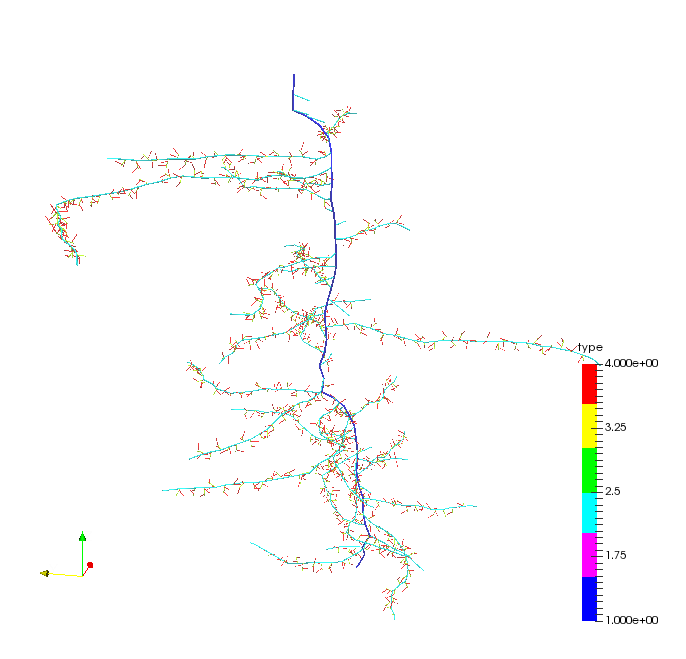
\includegraphics[width=0.99\textwidth]{example_1a.png}
\subcaption{Unconfined growth (Example 1a)} \label{fig:basicA}
\end{subfigure}
\begin{subfigure}[c]{0.5\textwidth}
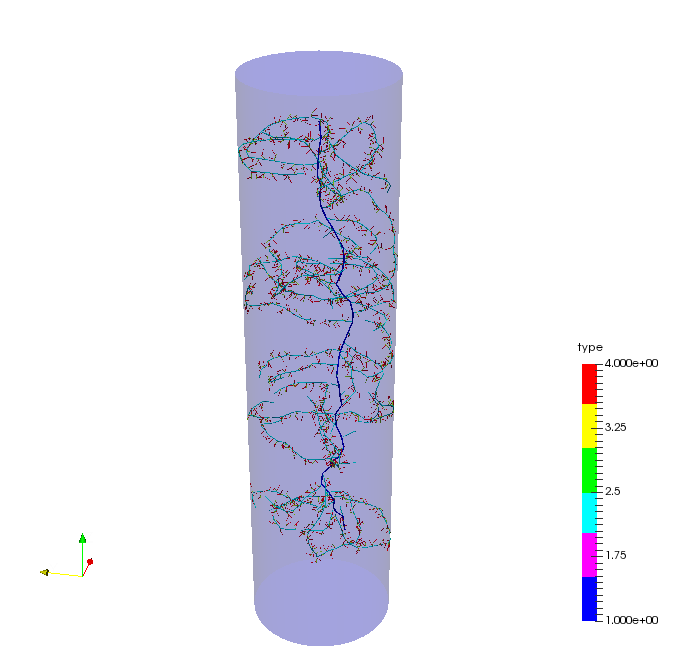
\includegraphics[width=0.99\textwidth]{example_1b.png}
\subcaption{Confined to soilcore (Example 1b)} \label{fig:basicB}
\end{subfigure}
\caption{Paraview visualizations of results of example 1a and 1b.} 
\end{figure}

Next, we show how to build more complex container geometries using SDF, 
furthermore, we show an example with multiple root systems that is computed in parallel.

\subsection{Using SDF with set operations}

In the following example we create geometries that we might encounter in experiments. 
First, we show how to rotate a rhizotron (e.g. to see more roots at the wall due to gravitropism). 
Second, we create a split box experiment, and furthermore, an example where rhizotubes act as obstacles.

The following examples demonstrates how to build a complex geometry using rotations, translations and set operations on the SDF.

\lstinputlisting[language=Python, caption=Example 1c]{../../examples/python/example1c_complexcontainer.py}

\begin{itemize}

\item[15-21] Definition of a rotated rhizotron, see Figure \ref{fig:rhizo}: 
L17 creates the flat container with a small height, this container is then rotated and translated into the desired position. 
L18 is the position where the origin will lie, and L19 the rotational matrix around the x-axis. 
In L20 the origin position is rotated. Finally, in L21 the new rotated and translated geometry is created. 
\item[23-32] Definition of of a split box, see Figure \ref{fig:split}: 
The split box is composed of a left box, a right box, and a top box connecting left and right. 
In L31 the geometry is defined by the set operation union of the three compartments. 
\item[34-49] Definition of rhizotubes as obstacles, see Figure \ref{fig:rhizotubes}: L35 is the surrounding box, 
L36 a single rhizotube, that is rotated around the y-axis in L37. 
L39-L46 create a list of rhizotubes at different locations that mimics the experimental setup. 
L48 and L49 compose the final geometry by to set operation, first a union of all tubes, 
and then cut them out the surrounding box by taking the difference. 
\item[52] Pick one of the three geometries for your simulation.
\item[62] Also more complex geometries can be visualized by the Paraview script, 
however, set operations are not really performed, only the involved geometries are visualized.
\item[65] As before we cannot visualize the container geometry in the interactive rendering, but only the roots. We give two additional arguments: The first argument 'True' indicates that an interactive window should be created, otherwise with 'False' we are only interested in the return value of the method. The second argument is the axis alignhment. Currently, the options are 'top\_view', 'side\_view' (default), or 'oblique'. 

\end{itemize}

% TODO describe the creation of hte paraview plots in detail...


\begin{figure}
\begin{subfigure}[c]{0.3\textwidth}
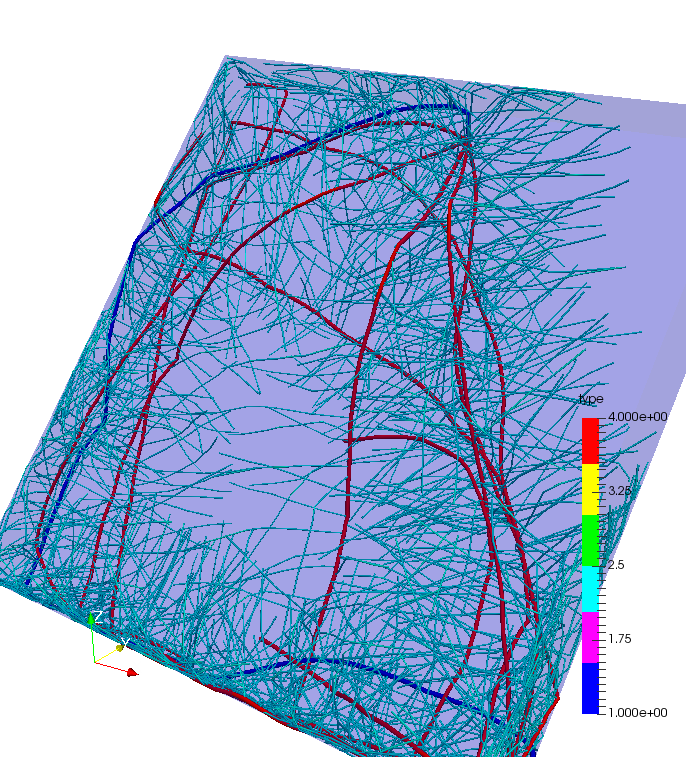
\includegraphics[width=0.99\textwidth]{example_2a1.png}
\subcaption{Rotated rhizotron} \label{fig:rhizo}
\end{subfigure}
\begin{subfigure}[c]{0.3\textwidth}
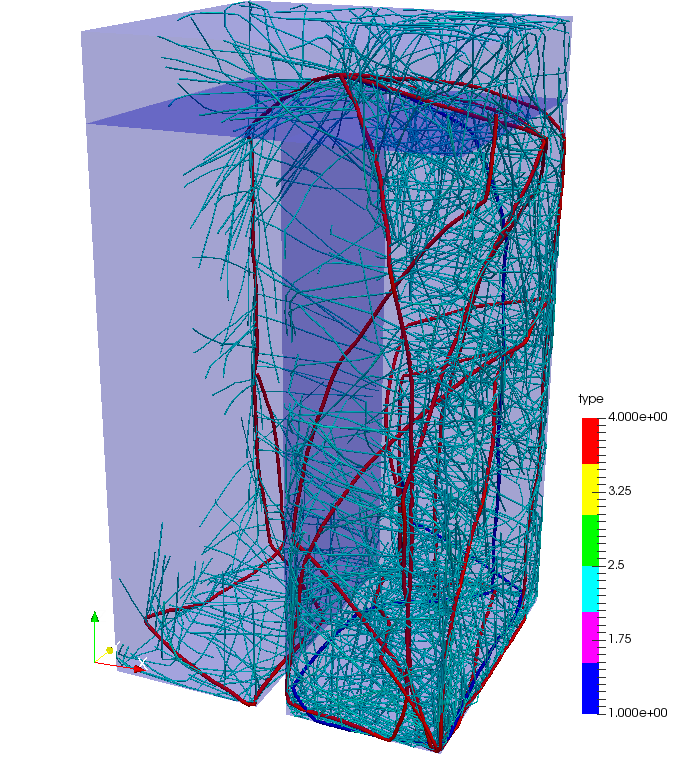
\includegraphics[width=0.99\textwidth]{example_2a2.png}
\subcaption{Split box} \label{fig:split}
\end{subfigure}
\begin{subfigure}[c]{0.3\textwidth}
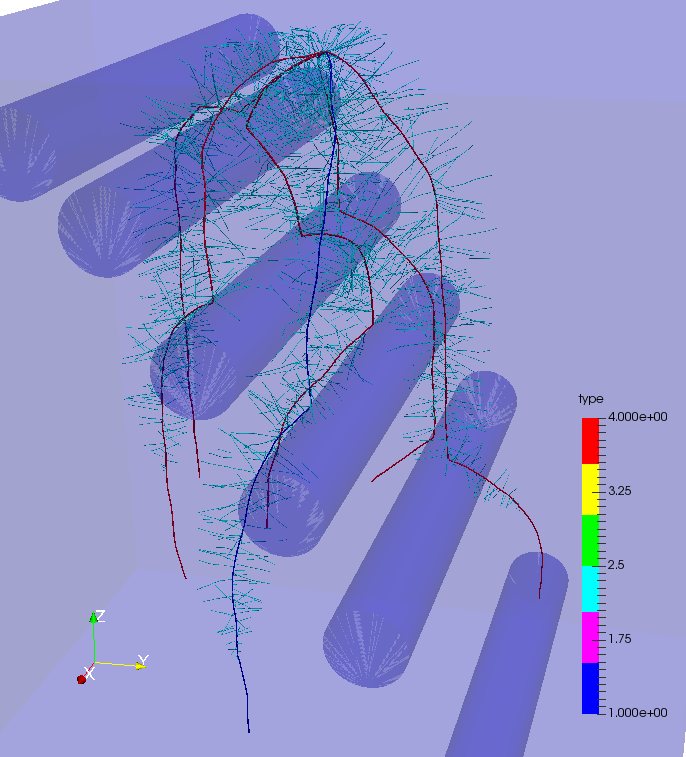
\includegraphics[width=0.99\textwidth]{example_2a3.png}
\subcaption{Rhizotubes} \label{fig:rhizotubes}
\end{subfigure}
\caption{Different geometries described by SDF (Example 1c)}
\end{figure}

\subsection{Multiple root systems}

Its possible to simulate multiple root systems. In the following we show a small plot scale simulation.

\lstinputlisting[language=Python, caption=Example 1d]{../../examples/python/example1d_multiple.py}

\begin{itemize}

\item[11,12] Set the number of columns and rows of the plot, and the distance between the root systems.

\item[15-22] Creates the root systems, and puts them into a list allRS. L20 sets the position of the seed. 

\item[25,26] Simulate all root systems 

\item[29-36] Saves each root systems, and additionally, saves all root systems into a single file. 
Therefore, we create an SegmentAnalyser (see Section \ref{sec:sa}) object in L29 and merge all segments into it L33, 
and finally export the single file L36. The resulting geometry is shown in Figure \ref{fig:multiple}.

\end{itemize}

If we consider only one plant type we often simplify plot scale simulations to a single plant simulation with periodic boundary conditions. We can analyse the root geometry with an underlying periodic grid as described in Section \ref{ssec:periodic}. 

\begin{figure}
\centering
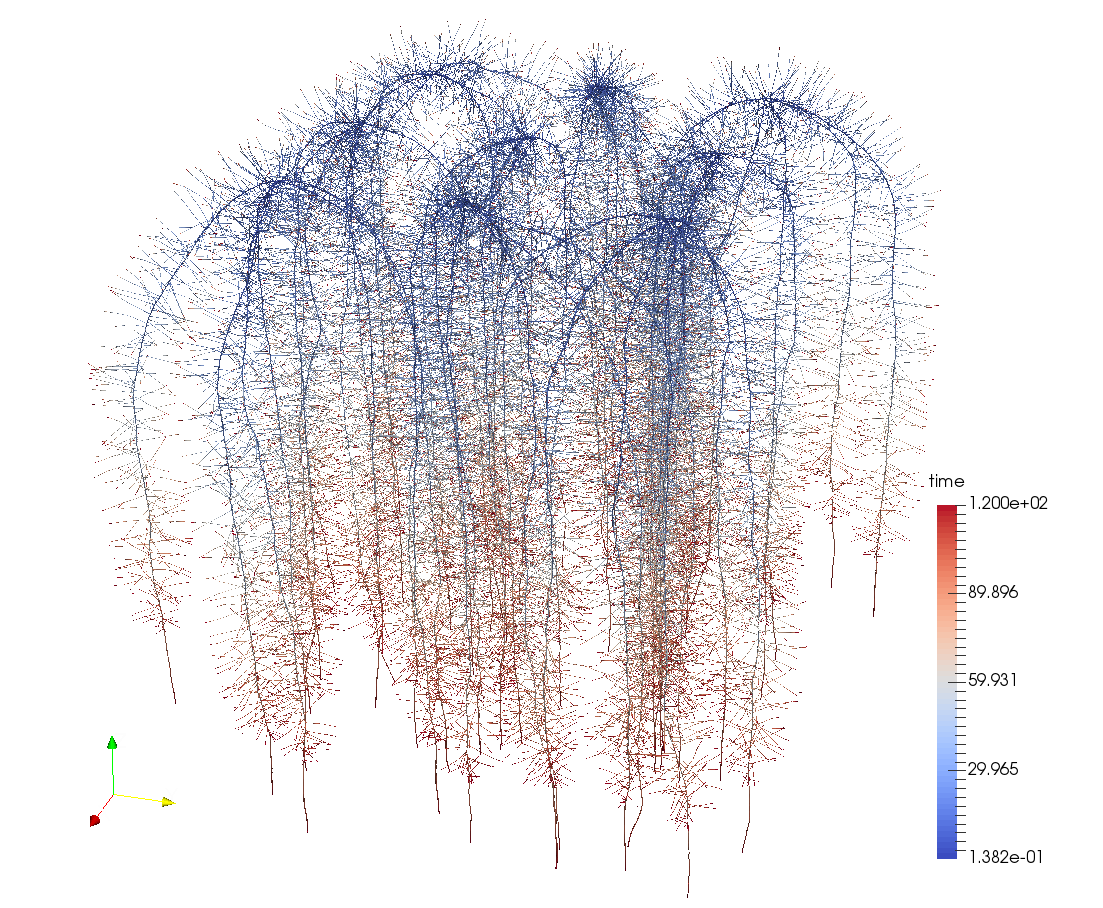
\includegraphics[width=0.7\textwidth]{example_2b.png}
\caption{Multiple root systems (Example 1d), colors denote the creation time of the root segments} \label{fig:multiple}
\end{figure}
